\section[Introduzione]{Introduzione}
\sectionframe{images/covers/cover_intro.jpg}{Introduzione}

\subsection[Introduzione]{Introduzione}

% Pastorello: intro_statistical_learning
% https://www.javatpoint.com/machine-learning
\begin{frame}
	% \frametitle{Introduzione}
	
	\begin{block}{Introduzione}
		\begin{itemize}
				\item Nel mondo reale, siamo circondati da esseri umani che possono imparare tutto dalle loro esperienze con la loro capacità di apprendimento.
				\item Noi umani sappiamo svolgere task molto complessi che vanno al di là di quello che riusciamo a spiegare.\\
					Esempi classici sono:
					\begin{itemize}
						\item[--] riconoscere volti
						\item[--] riconoscere immagini
						\item[--] riconoscere cifre o parole scritte a mano
					\end{itemize}
				\item Come possiamo addestrare un computer a svolgere questi compiti al posto nostro? Sicuramente non con una sequenza di if, then, else\ldots
				\item Ma una macchina può imparare anche dalle esperienze o dai dati passati come fa un essere umano?\\ 
			\end{itemize}
		La risposta è sì.\\
		Il \mlbold nasce per svolgere alcuni di questi task.
	\end{block}
\end{frame}


\subsection[Definizione]{Definizione}
% https://www.javatpoint.com/machine-learning
% Ottavio Calzone: Pagina 21-42 definizione ML
\begin{frame}
	%\frametitle{Definizione}
	
	\begin{block}{Definizione}
		Il \mlbold è una tecnologia in espansione che consente ai computer di apprendere automaticamente da dati precedentemente raccolti.
		
		\begin{figure}[!htbp]
			\centering
			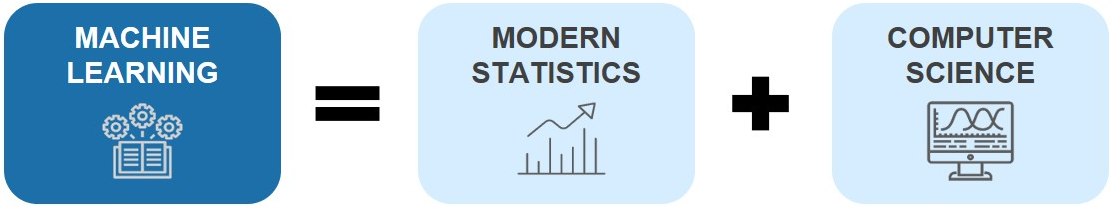
\includegraphics[width=0.6\linewidth]{images/intro/machine_learning_definition.png}
			%\caption{Stripe Radar for Fraud Detection}
		\end{figure}
		
		Attraverso l'uso dei dati storici di esempio, gli algoritmi di \ml riuniscono \textbf{informatica e statistica} per creare \textbf{modelli matematici} che aiutano a fare \textbf{previsioni} o prendere \textbf{decisioni} senza essere stato programmato esplicitamente.
		
		\begin{figure}[!htbp]
			\centering
			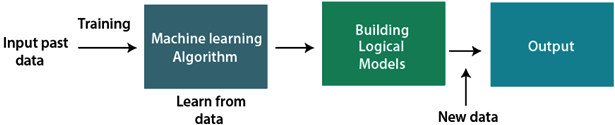
\includegraphics[width=0.73\linewidth]{images/intro/introduction-to-machine-learning.png}
		\end{figure}
	\end{block}
	
\end{frame}


\subsection[Contesto]{Contesto}
\begin{frame}
	%\frametitle{Definizione}
	
	\begin{block}{Contesto}
		Talvolta i due termini \textbf{Artificial Intelligence} (AI) e \mlbold (ML) vengono utilizzati erroneamente come sinonimi.\\
		Queste due tecnologie sono correlate tra loro, entrambe sono utilizzate per la creazione di sistemi intelligenti.\\
		Ad un livello più ampio, possiamo differenziare sia AI che ML in quanto:
		\begin{itemize}
			\item L'AI è un concetto più ampio per creare macchine intelligenti in grado di simulare capacità e comportamenti del pensiero umano,
			\item Mentre l'ML è un'applicazione o un sottoinsieme della AI che consente alle macchine di apprendere dai dati senza essere state programmato esplicitamente.
		\end{itemize}
	
	\end{block}
	
\end{frame}


\begin{frame}
	%\frametitle{Definizione}
		
	\begin{figure}[!htbp]
		\centering
		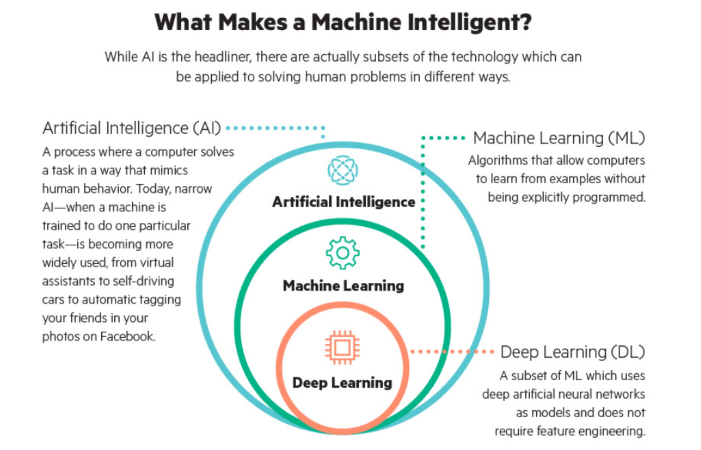
\includegraphics[width=12.0cm]{images/intro/ai_ml_dl.png}
	\end{figure}
	
\end{frame}


\subsection[Applicazioni]{Applicazioni}
\begin{frame}
	
	%\frametitle{1.0 Scopo}
	\begin{figure}[!htbp]
		\centering
		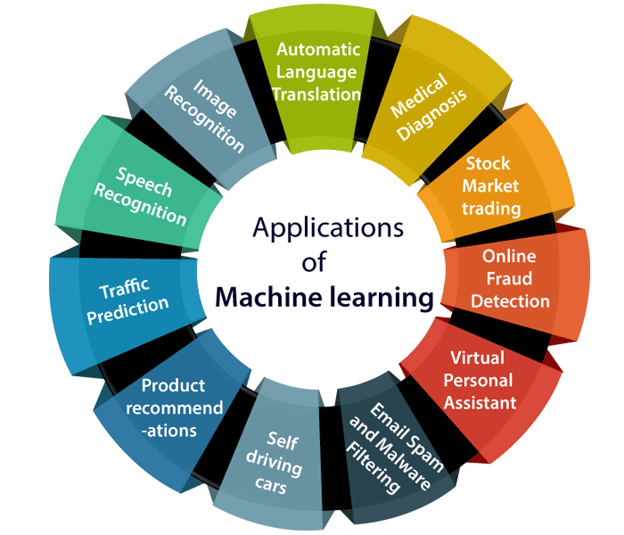
\includegraphics[width=9.0cm]{images/intro/ml_applications.png}
	\end{figure}

\end{frame}


\begin{frame}
	
	\frametitle{Applicazioni}
	%\begin{block}{}
		\begin{itemize}
			\item \textbf{Riconoscimento di immagini}:\\
				Il riconoscimento delle immagini è una delle applicazioni più comuni dell'apprendimento automatico. Viene utilizzato per identificare oggetti, persone, luoghi, immagini digitali, ecc\dots
			\begin{figure}[!htbp]
				\centering
				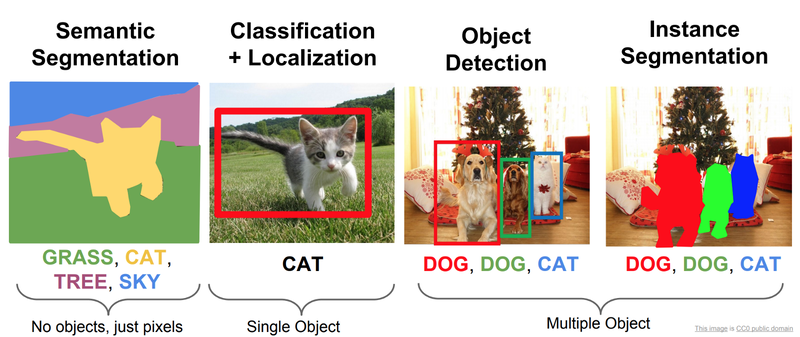
\includegraphics[width=11.0cm]{images/intro/ml_image_recognition.png}
			\end{figure}
			
		\end{itemize}		
	%\end{block}

\end{frame}

\begin{frame}
	
	\frametitle{Applicazioni}
	%\begin{block}{}
		\begin{itemize}
			\item \textbf{Riconoscimento vocale}:\\
				Il riconoscimento vocale è un processo di conversione delle istruzioni vocali in testo, spesso indicato come \textbf{Speech to Text} (STT) o \textbf{Computer Speech Recognition}. Al momento sono ampiamente utilizzati da varie applicazioni di riconoscimento vocale come:
				 	\begin{itemize}
				 		\item Google Assistant
				 		\item Siri
				 		\item Cortana
				 		\item Alexa
				 	\end{itemize}
			\begin{figure}[!htbp]
				\centering
				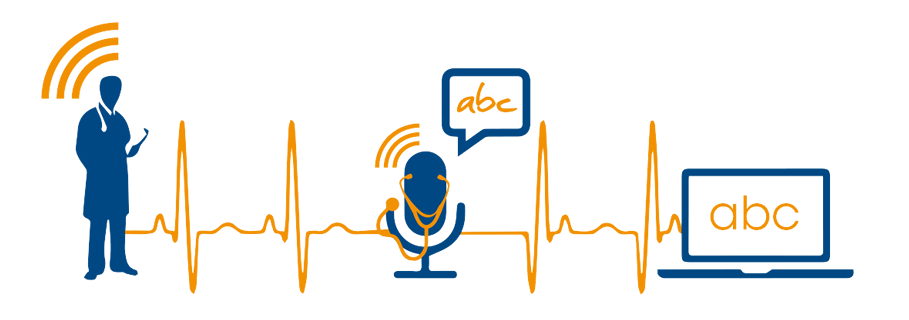
\includegraphics[width=7.5cm]{images/intro/speech_recognition.png}
			\end{figure}
			
		\end{itemize}		
	%\end{block}

\end{frame}


\begin{frame}
	
	\frametitle{Applicazioni}
	%\begin{block}{}
		\begin{itemize}
			\item \textbf{Previsioni del traffico}:\\
				Se ci avvaliamo dell'aiuto di \textit{Tom Tom} o \textit{Google Maps} per visitare un luogo, ci viene indicato il percorso più breve con una indicazione circa le condizioni del traffico. 
				Riescono a predire se il traffico è assente, presente o fortemente congestionato con l'aiuto di informazioni incrociate: 
				\begin{itemize}
				 		\item la posizione in tempo reale del veicolo (app + sensore gps)
				 		\item tempo medio di percorrenza dello stesso percorso negli ultimi giorni nella stessa fascia oraria
				 	\end{itemize}
				Tutti coloro che utilizzano questi servizi aiutano i providers a migliorare le proprie applicazioni.
				Prendono le informazioni dall'utente e le rimandano al rispettivo database per migliorarne le prestazioni.
				 	
			\begin{figure}[!htbp]
				\centering
				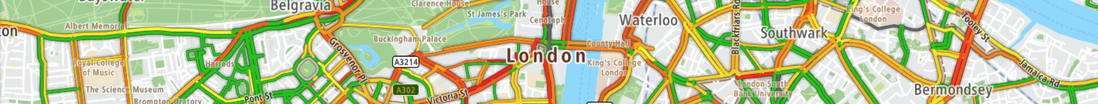
\includegraphics[width=10cm]{images/intro/tom_tom_traffic.png}
			\end{figure}
			
		\end{itemize}		
	%\end{block}

\end{frame}



\begin{frame}
	
	\frametitle{Applicazioni}
	%\begin{block}{}
		\begin{itemize}
			\item \textbf{Raccomandazioni}:\\
				Il ML è ampiamente utilizzato da varie società di e-commerce e intrattenimento come Amazon, Netflix, ecc \\
				per la raccomandazione di prodotti o film si cerca di comprendere gli interessi dell'utente utilizzando vari algoritmi di ML, quindi si tenta di suggerire un nuovo item sulla base di tali interessi.
				\begin{figure}[!htbp]
					\centering
					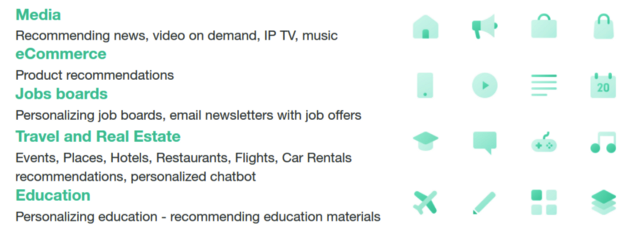
\includegraphics[width=10.5cm]{images/intro/recommendations_examples.png}
				\end{figure}
		\end{itemize}		
	%\end{block}

\end{frame}


\begin{frame}
	
	\frametitle{Applicazioni}
	%\begin{block}{}
		\begin{itemize}
			\item \textbf{Auto a guida autonoma}:\\
				Una delle applicazioni più interessanti dell'apprendimento automatico sono le auto a guida autonoma.\\
				%Tesla, la più famosa azienda produttrice di auto, sta lavorando su auto a guida autonoma. Utilizza un metodo di apprendimento senza supervisione per addestrare i modelli di auto a rilevare persone e oggetti durante la guida.
				
				\begin{columns}
							
					\column{0.5\linewidth}
					\begin{figure}[!htbp]
						\centering
						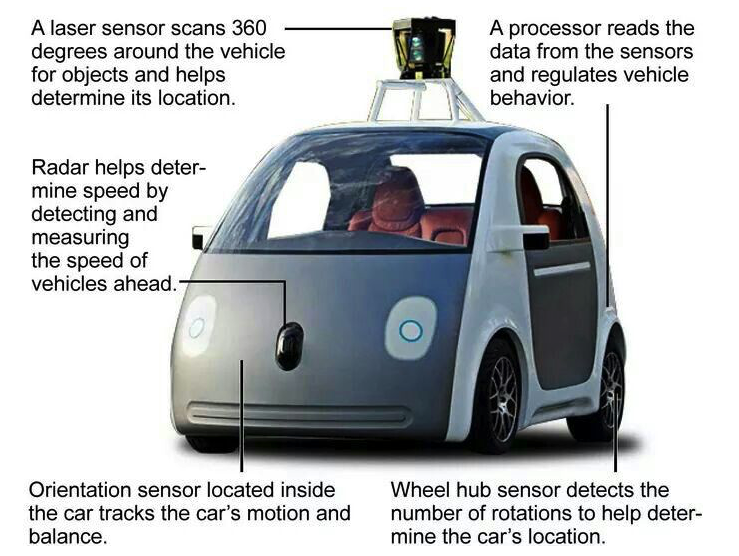
\includegraphics[angle=0,width=\linewidth]{images/intro/self_driving_car_google.jpg}
						\caption{Google Self Driving Car}
						%\label{Enel_HistFit_Normal} 
					\end{figure}
								
					\column{0.5\linewidth}
					\begin{figure}[!htbp]
						\centering
						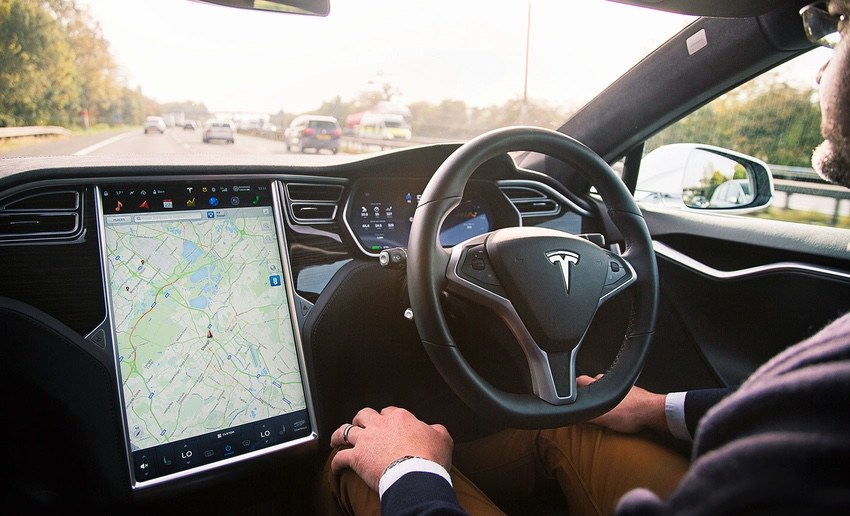
\includegraphics[angle=0,width=\linewidth]{images/intro/self_driving_car_tesla_autopilot.jpg}
						\caption{Tesla Auto Pilot}
						%\label{Enel_QQ_Plot_Normal} 
					\end{figure}
							
				\end{columns}

		\end{itemize}		
	%\end{block}

\end{frame}

\begin{frame}
	\frametitle{Applicazioni}
	%\begin{block}{}
		\begin{itemize}
			\item \textbf{Filtro antispam e malware per e-mail}:\\
				Ogni volta che riceviamo una nuova e-mail, viene automaticamente filtrata come importante, normale o spam. La posta elettronica è un modo efficiente per scambiare informazioni. Considerando la crescita di Internet e l'ampio utilizzo della posta elettronica, il tasso di aumento dello spam è motivo di grande preoccupazione.
				\begin{figure}[!htbp]
					\centering
					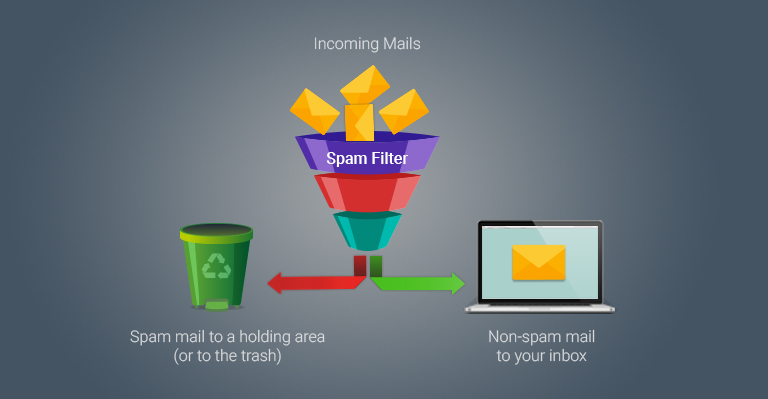
\includegraphics[width=7.5cm]{images/intro/anti-spam-filtering-techniques.jpg}
				\end{figure}
		\end{itemize}		
	%\end{block}
\end{frame}


\begin{frame}
	\frametitle{Applicazioni}
	%\begin{block}{}
		\begin{itemize}
			\item \textbf{Virtual Personal Assistant}:\\
				Esistono vari assistenti personali virtuali come Google Assistant, Alexa, Cortana, Siri, etc...\\
				Semplicemente con le nostre istruzioni vocali possiamo ordinare a questi dispositivi di riprodurre musica, chiamare qualcuno, aprire un'email, pianificare un appuntamento, ed altro.
				% Registrano le nostre istruzioni vocali, le inviano tramite su un servizio cloud dove vengono decodificate utilizzando algoritmi ML ed infine agiscono di conseguenza.
				\begin{figure}[!htbp]
					\centering
					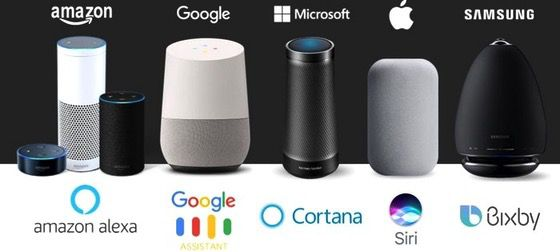
\includegraphics[width=8.5cm]{images/intro/assistants-vocaux.jpg}
				\end{figure}
		\end{itemize}		
	%\end{block}
\end{frame}


\begin{frame}
	\frametitle{Applicazioni}
	%\begin{block}{}
		\begin{itemize}
			\item \textbf{Rilevamento di frodi online}:\\
				Il ML sta rendendo le transazioni online più sicure e protette rilevando le transazioni fraudolente. Ogni volta che eseguiamo una transazione online, ci possono essere vari modi in cui può avvenire una transazione fraudolenta come account falsi, ID falsi o a metà di una transazione.
				%Quindi, per rilevarlo, possiamo avvalerci di questi strumenti che ci permettono di verificare se si tratta di una transazione autentica o di una transazione fraudolenta.\\
				
				\begin{figure}[!htbp]
					\centering
					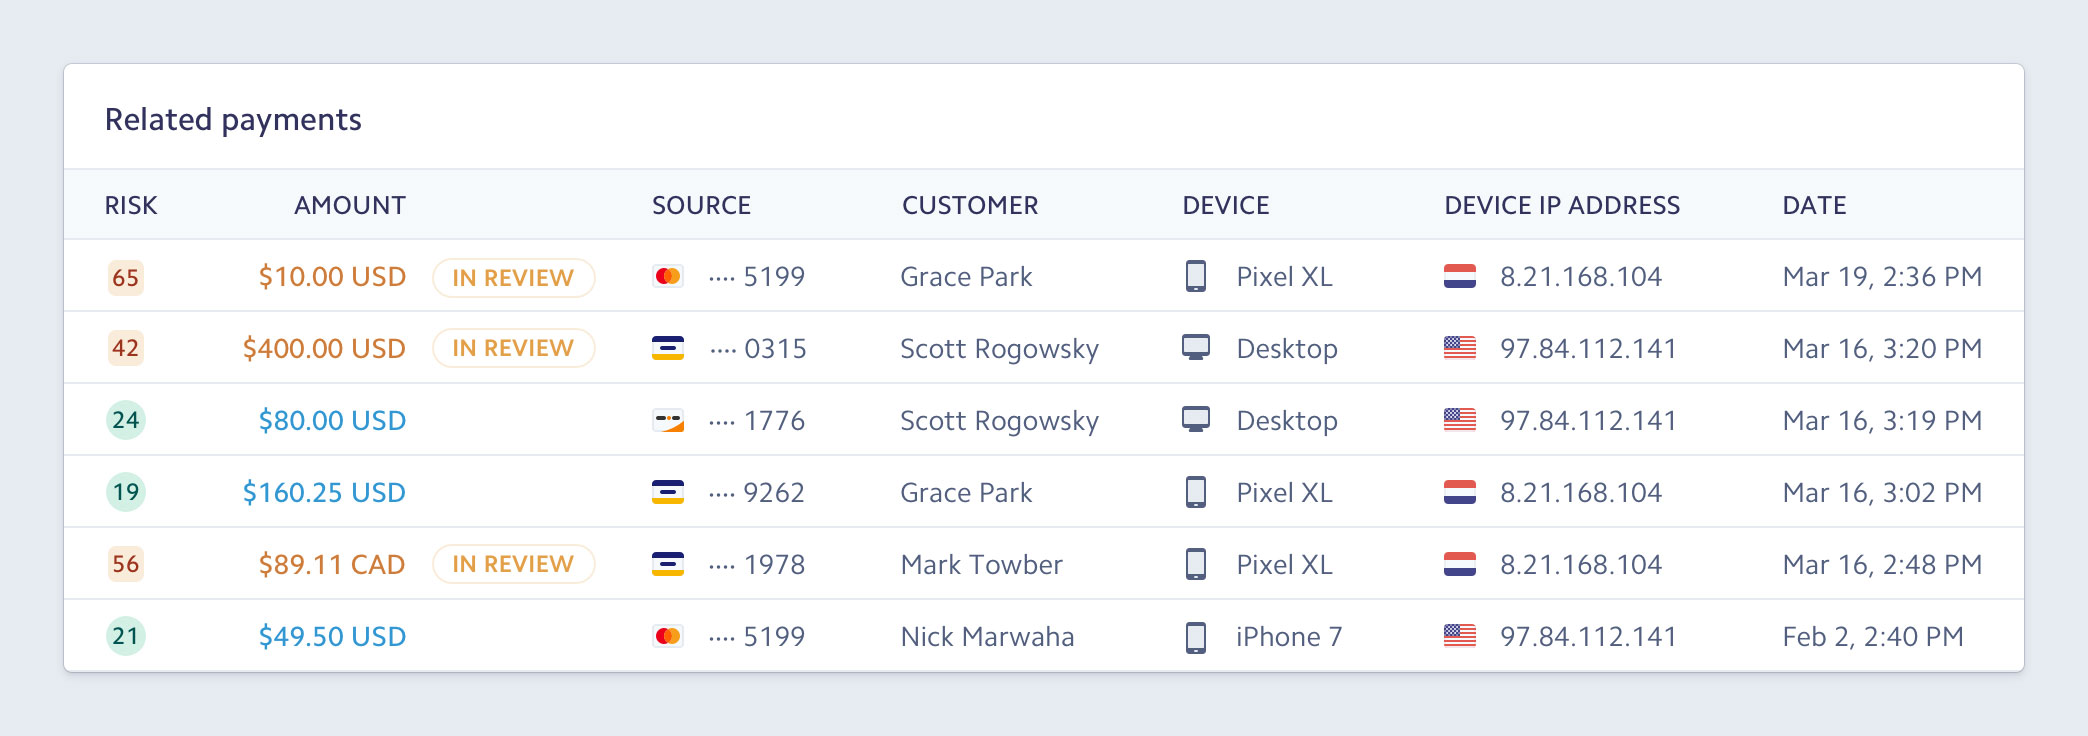
\includegraphics[width=9.5cm]{images/intro/stripe_radar.jpg}
					\caption{Stripe Radar for Fraud Detection}
				\end{figure}
		\end{itemize}		
	%\end{block}
\end{frame}



\begin{frame}
	\frametitle{Applicazioni}
	%\begin{block}{}
		\begin{itemize}
			\item \textbf{Trading}:\\
				L'apprendimento automatico è ampiamente utilizzato nel trading in borsa.\\
				Nel mercato azionario i prezzi delle azioni sono in continuo movimento.\\
				Il ML viene utilizzato per prevedere possibili trend di mercato oppure all'interno di trading systems automatici per generare ordini di compravendita automatici.
				\begin{figure}[!htbp]
					\centering
					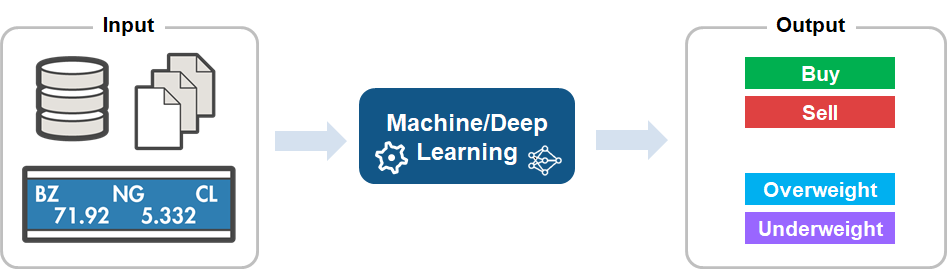
\includegraphics[width=10.5cm]{images/intro/ml_in_trading.png}
					%\caption{Stripe Radar for Fraud Detection}
				\end{figure}
		\end{itemize}		
	%\end{block}
\end{frame}


\begin{frame}
	\frametitle{Applicazioni}
	%\begin{block}{}
		\begin{itemize}
			\item \textbf{Diagnosi medica}:\\
				Nella scienza medica, il ML viene utilizzato per la diagnosi di alcune malattie.\\
				La tecnologia medica sta crescendo molto velocemente ed è ora in grado di costruire modelli 3D in grado ad esempio di localizzare l'esatta posizione di lesioni nel cervello (ad esempio tumori celebrali o altre malattie correlate al cervello).
				\begin{figure}[!htbp]
					\centering
					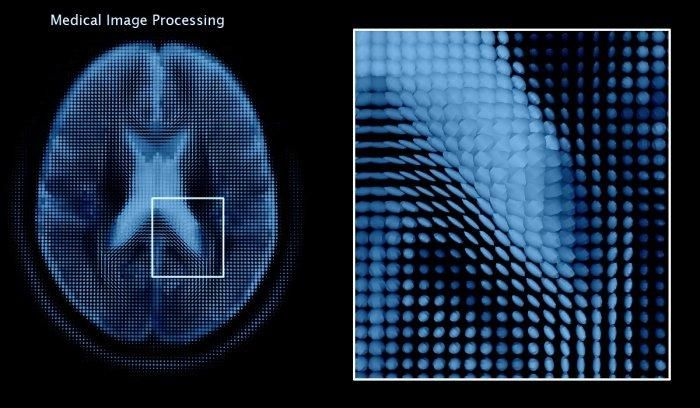
\includegraphics[width=5.7cm]{images/intro/medical_image_processing.jpg}
					%\caption{Stripe Radar for Fraud Detection}
				\end{figure}
		\end{itemize}		
	%\end{block}
\end{frame}


\begin{frame}
	\frametitle{Applicazioni}
	%\begin{block}{}
		\begin{itemize}
			\item \textbf{Traduzioni automatiche}:\\
				Al giorno d'oggi, se visitiamo un posto nuovo e non siamo a conoscenza della lingua allora non è affatto un problema.\\
				Ad esempio il GNMT di Google (Google Neural Machine Translation) fornisce questa funzionalità, traduce il testo nella nostra lingua.
				
				\begin{columns}
							
					\column{0.5\linewidth}
					\begin{figure}[!htbp]
						\centering
						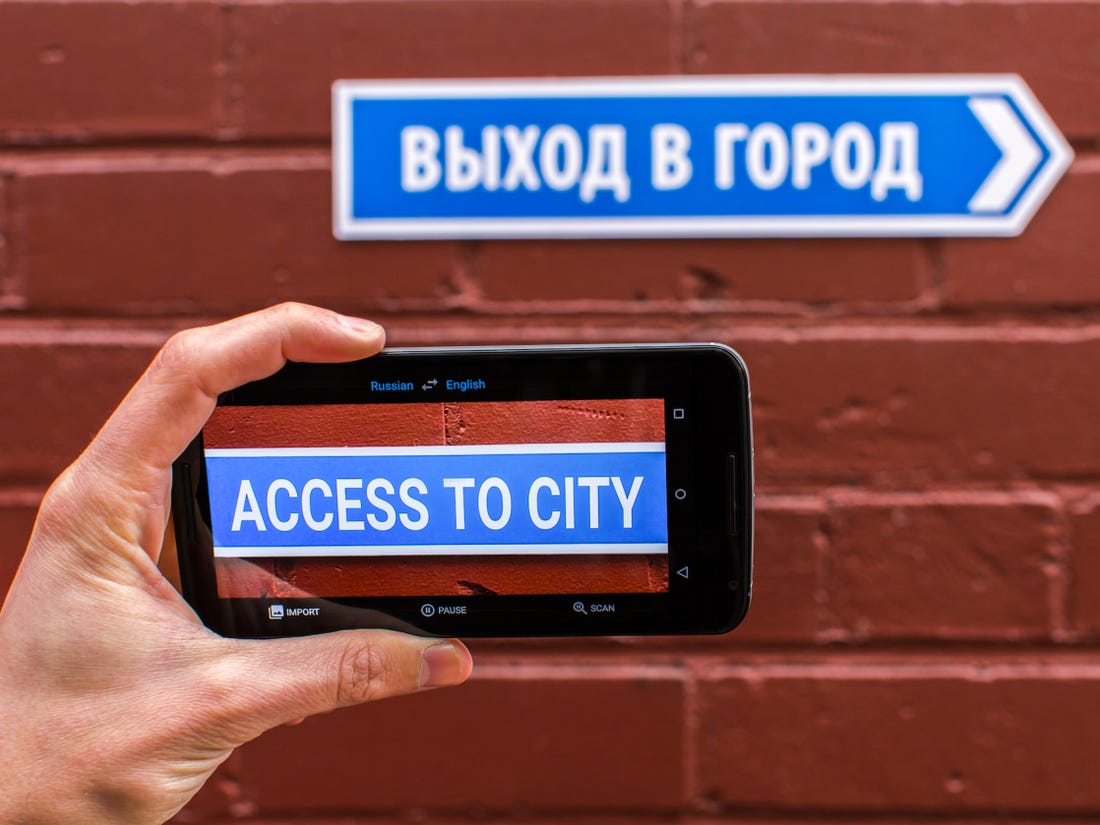
\includegraphics[angle=0,width=\linewidth]{images/intro/ml_gtranslate_1.jpeg}
						%\caption{Google Self Driving Car}
						%\label{Enel_HistFit_Normal} 
					\end{figure}
								
					\column{0.5\linewidth}
					\begin{figure}[!htbp]
						\centering
						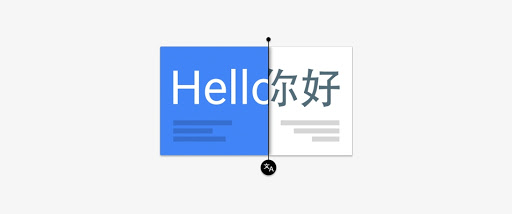
\includegraphics[angle=0,width=\linewidth]{images/intro/ml_gtranslate_2.jpeg}
						%\caption{Tesla Auto Pilot}
						%\label{Enel_QQ_Plot_Normal} 
					\end{figure}
							
				\end{columns}
			\end{itemize}		
	%\end{block}
\end{frame}


\begin{frame}
	
	%\frametitle{1.0 Scopo}
	\begin{figure}[!htbp]
		\centering
		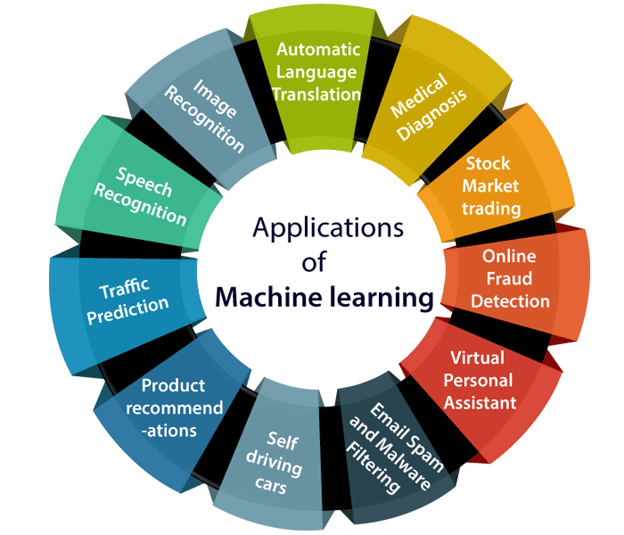
\includegraphics[width=9.0cm]{images/intro/ml_applications.png}
	\end{figure}

\end{frame}